% #############################################################################
% This is Chapter 5
% !TEX root = ../main.tex
% #############################################################################
% Change the Name of the Chapter i the following line
\fancychapter{Implementation}
\cleardoublepage
% The following line allows to ref this chapter
\label{chap:implementation}

This section builds on the system architecture. It will start by describing the communication protocols for each operation introduced in chapter \ref{chap:arch}, used in the implementation. The last section lists the standards and libraries chosen for the implementation. It finishes by outlining the implementation details, choices and their rationale.

% -----------------------------------------------------
% -----------------------------------------------------
\section{Protocol}\label{chap:implementation:protocol}

All data and operations will flow through a serial connection between the client software in the individual's computer and the physical box. A communications protocol needs to defined, in other for this communication to occur.
This section will explain and define the communication protocols between both the client application and the hardware device in detail. For each operation, it will describe its goal, the different phases, what data is traded in each phase and why.

% -----------------------------------------------------
\subsection{Initial State}\label{chap:implementation:protocol:initial-state}

The device will come from fabric configured and prepared with the necessary keys depending on two scenarios. In the simpler scenario, the device comes with the symmetric keys already shared and stored in each entities' device. They can begin to communicate immediately, with no setup necessary.
In the other scenario, the entities will receive the device with a pair of asymmetric keys, a private and public, generated inside the device from fabric. Each device will have the user's public keys, whom he wishes to communicate. The entity can request whose public keys he wants, before the device is initialized in fabric. This allows the users to share symmetric keys between them, which they can user to begin trading data securely.

All communications start with the client sending the operation code and receiving an "OK" message, meaning the user has access to the operation. If the user is not authenticated he receives a "NOT AUTHORIZED" message.
The authentication operation can always be be accessed by the user, all other operations can only be accessed after the user is authenticated.
Sending the operation code acts as a acknowledge message to check if the device is connected and powered to the computer.

% -----------------------------------------------------
\subsection{Authentication Protocol}\label{chap:implementation:protocol:auth}

Before executing any operation the user must authenticate himself to the device.
Figure~\ref{fig:protocol:authentication} depicts the authentication protocol.

%% ------------
\begin{figure}[h!]
	\centering     %%% not \center
	\subfigure[Authentication]{\label{fig:protocol:authentication}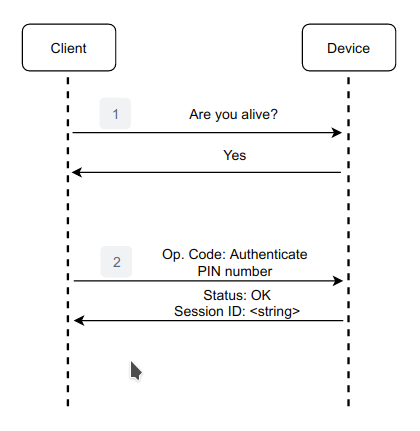
\includegraphics[width=70mm]{Images/authentication.png}}
	\subfigure[Change Authentication PIN]{\label{fig:protocol:change-PIN}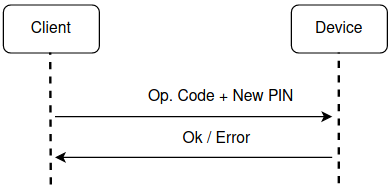
\includegraphics[width=70mm]{Images/change-PIN.png}}
	\caption{Authentication and PIN change protocols}
\end{figure}
% \begin{figure}[h!]
%         \centering
%         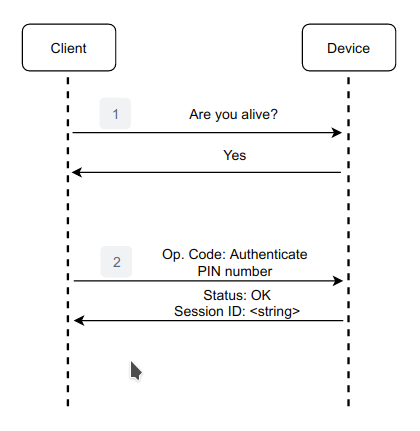
\includegraphics[width=0.4\textwidth]{./Images/authentication.png}
%         \caption{Authentication Protocol}
%         \label{fig:protocol:authentication}
% \end{figure}

The user initiates by sending a operation code. After the "OK" message, the user provides the device with the authentication \ac{PIN}. The device will respond with a authentication response parameter indicating failure or success. If successful, the session will be unlocked, allowing the user access to the main operations.

% -----------------------------------------------------
\subsection{Administration Protocol}\label{chap:implementation:protocol:admin}

There is only one administration operation, to change the authentication \ac{PIN}, pictured in figure~\ref{fig:protocol:change-PIN}.

% \begin{figure}[h!]
%         \centering
%         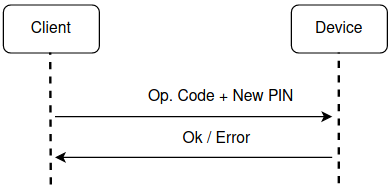
\includegraphics[width=0.4\textwidth]{./Images/change-PIN.png}
%         \caption{Protocol to Change Authentication PIN}
%         \label{fig:protocol:change-PIN}
% \end{figure}

After the operation code and received status message, the user sends the new \ac{PIN} number. The device responds with the status message of the operation.

% -----------------------------------------------------
\subsection{Secure Communications Protocol}\label{chap:implementation:protocol:comms}

The protocol for operations which secure communications will be defined here. It covers the encryption and authentication operation, which enables secure communications.% and non-repudiation through qualified digital signatures.
The protocol for secure data exchange illustrated in figure~\ref{fig:protocol:data-exchange} consists of four stages.

\[E_{k1}\{Data, IV\}\, MAC_{k1}\{IV+E_{k1}\{Data, IV\}\}\]

\[(MAC_{k1}\{IV+Ciphertext\} == MAC) => E_{k1}\{Ciphertext, IV\} => Data\] 

\begin{figure}[h!]
	\centering
	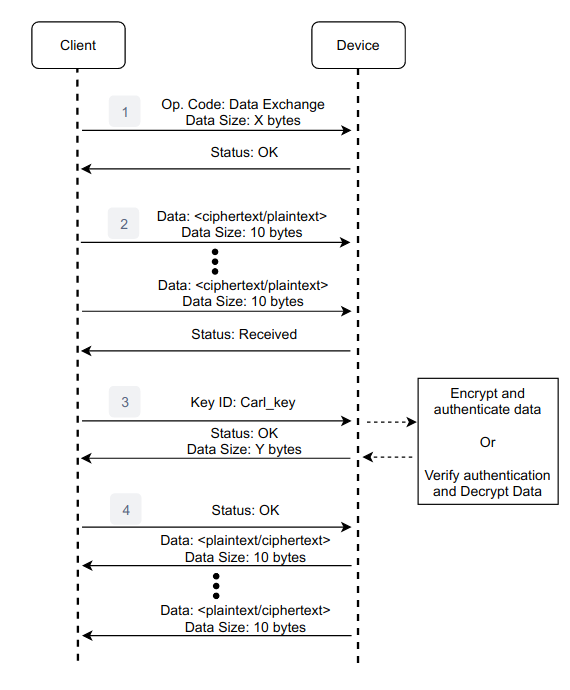
\includegraphics[width=0.55\textwidth]{./Images/data-exchange.png}
	\caption{Encryption+Authentication Protocol}
	\label{fig:protocol:data-exchange}
\end{figure}

The first stage is identical to all operations, the client sends the operation code and receives the authorization status. If he is not authorized, the user is required to authenticate first.
In the second stage the user client application sends the data size to be encrypted, waits for the "OK", and starts sending the data one block at a time.
A maximum of 16 bytes per message can be transmitted. Each message contains a part of the data and the size of the data in that packet. When the transmission ends, the device confirms its reception with an "OK" message.
In the third stage, the client software sends the ID of the symmetric key used to secure communications with.
In the final stage, after the box has finished the cryptographic operations, the device sends the result size to the client, waits for an "OK" message and sends the result. It consists of the encrypted data, MAC and IV.

The protocol to decrypt and authenticate is identical to the one pictured in figure~\ref{fig:protocol:data-exchange}. The device receives the ciphertext, \ac{MAC} and \ac{IV}, and returns the original plaintext data.

\hfill
\hfill

% The next protocols are relating to the generation and verification of digital signatures.
% The designed protocol for generation is represented in figure~\ref{fig:protocol:signature-generate}.
\[Sign_{K_A}\{Hash\{Data\}\}\]

%% ------------
% \begin{figure}[h!]
%         \centering     %%% not \center
%         \subfigure[Generation Protocol]{\label{fig:protocol:signature-generate}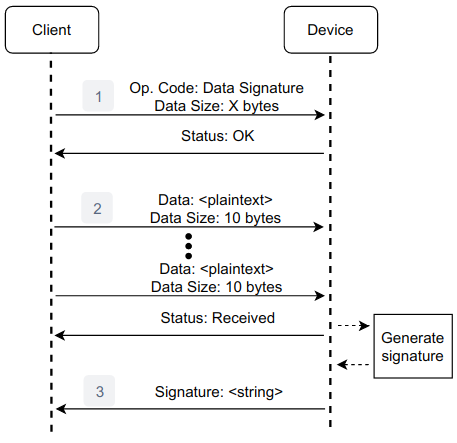
\includegraphics[width=79mm]{Images/signature-generate.png}}
%         \subfigure[Verification Protocol]{\label{fig:protocol:signature-verify}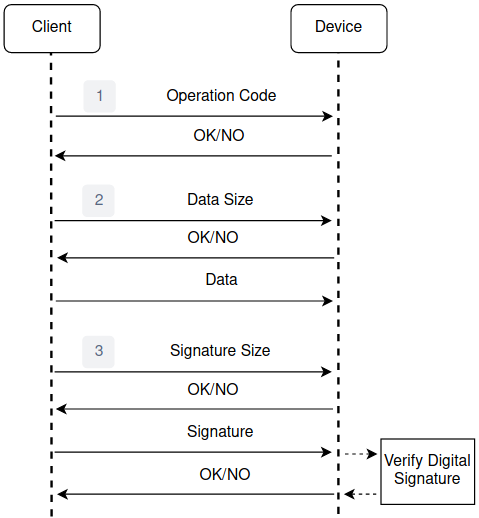
\includegraphics[width=79mm]{Images/signature-verify.png}}
%         \caption{Digital Signature Generation Protocols}
% \end{figure}

% The user initiates by sending the operation code and the plaintext data size.
% When the box responds with an OK message, the user transmits the data to be signed, one message at a time.
% In possession of the data, the device will generate the digital signature using the device's private key. When finished the signature is sent back to the user.
%
% The protocol for verifying digital signatures is pictured in figure~\ref{fig:protocol:signature-verify}.
% After the user sends the operation code, and the box responds with an OK message, the user transmits the data, used by the signer to generate the signature, one message at a time.
% When done, the user also sends the signature and the name of the signer, so the device knows what public key to use to verify the signature.
% Then, the device will verify the digital signature using the signer's public key, the data and the signature. The result will be sent back to the user.
%
% -----------------------------------------------------

\subsection{Communication Management Protocol}\label{chap:implementation:protocol:key}

The protocols for the communication management operations are detailed next, namely for symmetric key generation and key revocation. 
The protocol to generate a new symmetric key with another entity using asymmetric cryptography is detailed in figure~\ref{fig:protocol:ecdh}.

\[KDF\{ECDH_{K_B}\{K_A^{-1}\}, Salt\}\]

\[KDF\{ECDH_{K_A}\{K_B^{-1}\}, Salt\}\]

%% ------------
\begin{figure}[h!]
	\centering
	\subfigure[ECDH]{\label{fig:protocol:ecdh}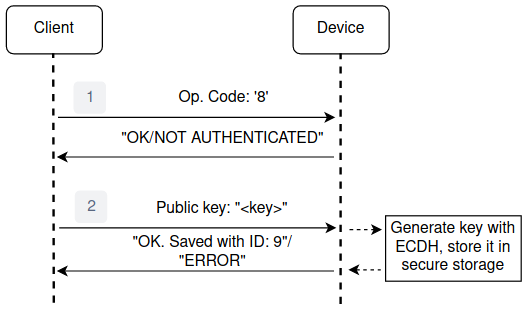
\includegraphics[width=79mm]{Images/ecdh.png}}
	\subfigure[Key Revocation]{\label{fig:protocol:delete-key}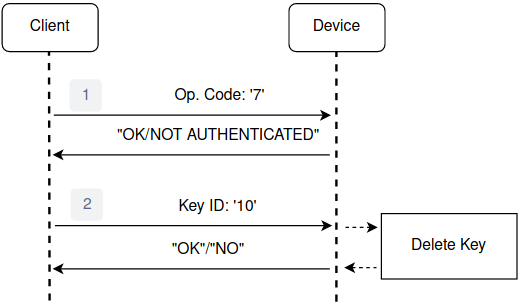
\includegraphics[width=79mm]{Images/delete-key.png}}
	\caption{Communication Management Protocols}
\end{figure}

After stage 1, the client forwards the entity's public key to the device, waits for an "OK" status, and sends the salt value. The device calls the ECDH algorithm with its private key and the received public key to generate a secret and run it through a key derivation function with the salt value to obtain the new symmetric key.
The new key is saved in secure storage with a new key id, which is returned to the client application.

The protocol for deleting an existing symmetric key from the device's secure storage is detailed in figure~\ref{fig:protocol:delete-key}.
After both sides trade operation code and OK status, the user sends the key ID, which identifies the symmetric key, and receives the operation status from the device after it has been deleted.

% -----------------------------------------------------
% -----------------------------------------------------
\section{Implementation}\label{chap:implementation:app}

This section contains all details about the developed implementation on the Hardware Security Module device and client interface.

% -----------------------------------------------------
\subsection{Libraries and Tools}\label{chap:implementation:app:tools}

The cryptographic software is running on the \ac{SoC} of a SmartFusion2 board, version M2S090TS from Microsemi, with the specifications described in section~\ref{chap:background:computing:smartfusion}. It is an adequate device due to several components such as the required cryptographic functions in its system controller, a \ac{TRNG} essential for cryptography, secure storage for keys and anti-tampering protections.
The application was implemented using the C programming language, with the SoftConsole v3.4 \ac{IDE} and libraries of the board functionalities, provided by Microsemi. The configuration was generated using Libero v11.7.
The device functions as a \ac{HSM}, connected through a \ac{USB} connection to a computer. It was programmed using the external FlashPro4 programmer required to develop and debug embedded applications with SoftConsole \cite{smartfusionSecurityPractices}.

% Mbedtls consideration
The inclusion of a cryptography library, such as Mbedtls, designed for embedded systems was considered. The library provides algorithm implementations: ECDH, ECDSA, AES encryption, HMAC and support for generation of X.509v3 certificates. The library can be integrated with the boards functionalities and have unnecessary features disabled to lower the used memory \cite{parrinha2017flexible}.
The paper compares the performance of operations on the smartfusion2 with the mbedtls library and the board's security cores. It concludes AES encryption has a higher throughput of 1.8 Mbit/s on the mbedtls implementation compared to the 730 Kbit/s on the embedded core. For the elliptic curve scalar multiplication, used for ECDH, the software implementation is significantly slower, from 28.4s per operation compared to 0.57s with the embedded core.
Ultimately, the security services offered by the device provide the necessary functionality to fulfill the requirements defined previously, with the exception of generating the device's certificate, but this was done by exporting the public key, generating the certificate and loading the certificate on the device.
Beyond increasing the memory footprint, the library does not offer significant performance benefits, or security measures against side-channel attacks similar to the one's offered by the device's services.

The client interface implemented the \ac{PKCS}\#11 standard for a higher device interoperability. The client interface was implemented in C++ for the open source MinGW compiler in Windows 10, and is composed of a simple command line interface which calls the implemented \ac{PKCS}\#11 interface functions based on the user's input.

% -----------------------------------------------------
\subsection{Communications}\label{chap:implementation:app:comms}

% The computer running the client interface and the smartfusion board, running the HSM code, are connected through a \ac{USB} connection with the external FlashPro4 programmer.
The device implementation uses the available \ac{UART} communication controller and corresponding drivers for communications.
It allows the board to send and receive messages of 16 block bytes at a time.
An abstraction layer on both ends was implemented to send and receive byte strings of any size with all the logic hidden.
When data of variable size is exchanged, such as plaintext and ciphertext, before transmission, the number of bytes is sent, so the receiver can validate and know how many bytes to expect.
In the case of fixed size data such as public keys and hashes this is not needed. For the remaining messages, which is usually a status message, all strings are terminated by the carriage return byte, so the receiver knows when the sender is done transmitting the message.

% -----------------------------------------------------
% \subsection{Cryptographic Algorithms}\label{chap:implementation:app:algorithms}
\subsection{Smartfusion Implementation}\label{chap:implementation:app:board}

The application in the device was implemented using several of the security services of the board: SRAM-PUF, AES, HMAC-SHA-256, ECC scalar point multiplication, KeyTree, \ac{NRBG} and tamper monitoring.

\subsubsection*{Authentication}

The authentication PIN is saved in the SRAM-PUF service in a predefined and static slot. When authentication is performed, the PIN is fetched, compared with the client's supplied PIN and erased from memory.
If the user is authenticated the PIN can be changed, by enrolling and overwriting the value in the PIN assigned SRAM-PUF slot.

\subsubsection*{Secure Communications}

As previously mentioned, the security of \ac{AES}-\ac{GCM} in hardware is considered to be unsurpassed by any authenticated-encryption scheme~\cite{aesmodes}.
Unfortunately, the SmartFusion2 board, does not support this encryption algorithm.
Therefore the solution implements a combination of an encryption algorithm with an authentication scheme. Among the supported \ac{AES} modes, as concluded in chapter~\ref{chap:background}, CTR mode is the most favourable option because of its efficiency and security, assuming the IV is unique for each message.

For authentication, the board supports \ac{HMAC} with the \ac{SHA}-256 hash function, which uses a 256 bit symmetric key and generates a 256 bit code. As concluded in section \ref{chap:background:crypto:mac}, it is a well-designed construction, even though it is not the most efficient.

For combining these algorithms, studies have shown that a combination of secure encryption and secure \ac{MAC} must use the encrypt-then-MAC method~\cite{encryptmacorder}.
Considering these guidelines, the data encryption/decryption and authentication implementation follows the protocol presented in figures~\ref{fig:arch-encrypt} and \ref{fig:arch-encrypt}.
The key used in HMAC should be different from the one used in encryption, to ensure the best security practices. So in practice, a key used for securing communications is split into two keys, one for encryption and one for authentication.
When choosing key sizes, taking into account the limited storage capacity of the board, a smaller, but still secure, key size is preferred. The \ac{AES} 128 bit or 256 bit services guarantee both 128 and 256 bit security. According to the \ac{NIST} recommendations~\cite{nistRecommendations}, algorithms which guarantee both 128 and 256 bit security, are expected to be secure from 2031 and beyond. Thus \ac{AES} with 128 bit keys is preferred, since it guarantees adequate security for the foreseeable future, and is the more conservative option.
Even though the HMAC service needs a 256 bit key, a 128 bit key can be used with the upper 128 bits padded with zeros \cite{smartfusionSecurityPractices}.
Therefore for every communication a 256 bit key is used, the lower 128 bits for encryption and upper 128 bits for authentication.

On encryption, a unique 16 byte \ac{IV} is generated using the \ac{NRBG} service.
The encryption and authentication keys, both 128 bit, are fetched from the SRAM-PUF service, using the slot (key ID) requested by the client application.
The returned string is either the original plaintext, or the \ac{MAC}, \ac{IV} and ciphertext, concatenated in that order.

% --------

% The system provides a single hash algorithm, \ac{SHA}-256, which has a security strength of 128 bits.
% The \ac{HMAC}-\ac{SHA}-256 algorithm needs a 256 bit key, different from the one used with encryption, to ensure the best security practices. A 128 bit key can be used, if padded with zeros. Thus, for every communication, a 128 bit key for encryption and a 128 bit key for authentication is used. In total, a 256 bit shared secret.

% The qualified digital signatures operation combines \ac{ECC} and the \ac{SHA}-256 hash algorithm, and provides 128 bit security, calculated by taking the smallest security strength value of both algorithms. For the encryption and authentication operation combining \ac{AES}-128 and \ac{HMAC}-\ac{SHA}-256, 128 bit security is provided.

% -----------------
\subsubsection*{Key Generation}
The supported \ac{ECC} P-384 curve guarantees 192 bit security.
The implemented new key generation operation protocol is defined in figures~\ref{fig:arch-ecdh-alice} and \ref{fig:arch-ecdh-bob}.
The peer's public key is supplied by the client application, and the device's private key is fetched from a predetermined PUF slot where it is saved.

For the ECDH algorithm the ECC scalar multiplication board accelerator is used. It multiplies a scalar value of 48 bytes, the private key, with a point with a x and y coordinate of both 48 bytes (96 bytes total), the public key.
The result is a 96 byte point, which is effectively the shared secret.
Then to generate the 256 bit key, the KeyTree service is applied as a key derivation function on the shared secret combined with a salt, which can be public.
The generated key is enrolled in the first available PUF slot, which is provided by a function in the API, and is returned to the user as the newly generated key ID.

\subsubsection*{Key Revocation}
Key revocation only consists of deleting the key from the SRAM-PUF slot it is saved. This is a simple call to the API function.

\subsubsection*{Tamper Detection}

Tamper and failure events detection is implemented. When certain events occur, flags are set which prevent the user from performing operations, to protect all possible sensitive data.
On tamper detection events, zeroization is performed on the device, erasing all keys and data from the device. This process either makes the board unusable or reset to the default fabric state.
These measures effectively have a denial-of-service effect but is a trade-off in order to avoid successful attacks and potential leaks of sensitive information, e.g. \ac{DPA}.

Using the AES and HMAC services, in the secure communications operation, which are not fully DPA-resistant, makes the keys and information vulnerable to these attacks, as discussed in section \ref{chap:background:computing:smartfusion}.
Attackers need physical access to the board and voltage measurement tools to perform them.
With the developed implementation using tamper detection, which blocks attackers from using the device and zeroization which erases all sensitive data from the device, helps mitigate this type of attacks.
All this is invalid, if the attacks somehow gain access to the user's authentication PIN.
Which is why regular replacement of symmetric keys used in the vulnerable operations is recommended, and is a missing feature of the implementation.
For future work a feature could be developed where a central entity, once every month, sends a encrypted message using pre-distributed keys, with a new key set, to replace the existing set.
% As discussed in section \ref{chap:background:computing:smartfusion}, physical access to the board is needed to perform these attacks

% TODO: maybe for conclusion: the secure communications service provides 128 bit security, and the ECDH algorithm provides 192 bit security.

% -----------------------------------------------------
\subsection{PKCS\#11 Interface}\label{chap:implementation:app:interface}

The application only supports one token and one session for the token.
PKCS\#11 defines two types of users, the regular user and security office. The implemented application does not make that distinction. Both types of user can login and perform operations.
The implemented application initializes the cryptoki application and opens the session with the device through the \texttt{C\_Initialize} and \texttt{C\_OpenSession} functions.
The opposite \texttt{C\_CloseSession} and \texttt{C\_Finalize} functions close the session and terminate the cryptoki application.

The interface handles the input from the user and uses the data to call the functions in the implemented PKCS\#11 API.
First the user inputs the operation code he wishes to perform, and the application handles the correct API calls to the PKCS\#11 interface.
The authentication operation calls the \texttt{C\_Login} function. The authentication PIN can then be changed with the \texttt{C\_SetPIN} function.
The \texttt{C\_Logout} function logs out the user. Only the operation code is needed for this operation.

To encrypt and authenticate some data, a local object for the secret key is created with \texttt{C\_CreateObject}. It does not contain the key data, only the key ID, so it can be passed of to the PKCS\#11 API. The encryption is performed through calls to \texttt{C\_EncryptInit} and then \texttt{C\_Encrypt}.
The same logic applied to decryption with \texttt{C\_DecryptInit} and then \texttt{C\_Decrypt}

For deleting a key on the device, first a secret key object is created with its ID, like before, and then a call to \texttt{C\_DestroyObject} handle the rest.
A new key is generated with the ECDH mechanism and \ac{SHA}-256 key derivation function, with a call to \texttt{C\_DeriveKey}.

Only one custom which is called directly is implemented. The \texttt{HSM\_C\_GetKeyList} returns the number of enrolled keys in the device.
% The solution should support a plethora of devices, as it will increase the adoptability of the solution among clients. This entails the use of a widely established protocol, which clearly defines a set of functions and standards the system should follow.
% The \ac{PKCS} \#11 standard will be utilized to fulfill this requirements. It allows operations to be standardized across different devices, increasing the range of supported devices. By implementing the system in accordance with these guidelines, it will have a higher device interoperability. Additionally, it allows the application to use, create and modify objects, without exposing them to its memory.
